\chapter{Analysis and Specifications}
\label{chap:analysis_specifications}

% ─────────────────────────────────────────────
\section*{Introduction}
\addcontentsline{toc}{section}{Introduction}
% ─────────────────────────────────────────────

This chapter evaluates the current enterprise recruitment methods, identifies their systemic limitations, and presents the distinctive advantages of our proposed platform. It then formally specifies the functional and non-functional requirements alongside global use case modeling.

\newpage

% ═══════════════════════════════════════════════
\section{Existing System Study}
\label{sec:existing_system_study}
% ═══════════════════════════════════════════════

% ──────────────────────────────────────────────
\subsection{Current Recruitment Methods}
\label{subsec:current_methods}
% ──────────────────────────────────────────────

Enterprise recruitment today relies on three dominant technology models, each with distinct operational characteristics:

\begin{itemize}
    \item \textbf{Commercial SaaS ATS Platforms} --- Workday Recruiting, Oracle Taleo, Greenhouse, iCIMS Talent Cloud
    \item \textbf{Legacy On-Premise ERP Modules} --- SAP HCM Personnel Administration, SAP Recruitment, SAP Organizational Management via SAP GUI
    \item \textbf{Hybrid Manual Workflows} --- Spreadsheet-based tracking, email-driven communication, disconnected document storage
\end{itemize}

While these approaches offer partial solutions --- SaaS platforms provide modern candidate portals and pipeline visualization, ERP modules ensure data consistency within the corporate system, and manual workflows offer flexibility --- they share a common set of structural deficiencies. SaaS platforms operate in isolation from the enterprise ERP core, forcing HR staff to manually re-enter candidate data after hiring, a slow and error-prone step on records that later feed payroll. Legacy SAP GUI screens are inaccessible to external candidates and offer \textbf{no self-service}. Resume screening relies either on manual reading or on rigid keyword matching, which can reject qualified candidates whose resumes do not use the expected words. Furthermore, any customization of on-premise ERP recruitment workflows requires invasive core modifications that violate SAP's Clean Core paradigm and generate significant technical debt.

% ──────────────────────────────────────────────
\subsection{Particularities of Our Solution}
\label{subsec:solution_particularities}
% ──────────────────────────────────────────────

Our platform addresses every limitation identified above through three architectural pillars:

\textbf{Native SAP BTP Clean Core Integration.} Upon HR approval, a single RAP action creates the employee master record and its child records from the verified onboarding data, in less than half a second in our measurements and without any manual re-entry. Built as a side-by-side extension on SAP BTP using ABAP Cloud and SAP HANA Cloud, the architecture leaves the standard ERP objects untouched, which keeps the core upgradable (Clean Core).

\textbf{AI-Assisted Resume Screening.} A Python microservice uses a large language model (GPT-4o-mini) to parse each resume into a structured profile, enrich it with the candidate's GitHub projects, and score it against the rubric of the role and the requirements of the job offer, with evidence for each criterion. The final score is computed deterministically in Python. The evaluation runs in the background, takes about half a minute to a minute per resume, and costs about 0.003~USD. Transparent per-criterion scores with natural-language justifications keep the recruiter in control of the decision.

\textbf{Dual Modern User Experience.} A responsive React/Vite candidate portal enables job discovery, one-click application, real-time pipeline tracking, and onboarding self-service. An enterprise SAP Fiori Elements cockpit equips recruiters with draft handling, configurable pipelines, and one-click stage progression.

\subsection{Comparative Synthesis}
\label{subsec:comparative_synthesis}

\begin{table}[H]
\centering
\caption{Comparative Analysis --- Current Methods vs.\ Our Proposed Solution}
\label{tab:comparative_synthesis}
\renewcommand{\arraystretch}{1.4}
\small
\begin{tabular}{|>{\raggedright\arraybackslash}p{3.5cm}|>{\raggedright\arraybackslash}p{3cm}|>{\raggedright\arraybackslash}p{3cm}|>{\raggedright\arraybackslash}p{4.2cm}|}
\hline
\textbf{Dimension} & \textbf{SaaS ATS} & \textbf{Legacy SAP GUI} & \textbf{Our Solution} \\
\hline
ERP Data Integration & Isolated silo, manual re-entry & Native but internal only & \textbf{Native \& decoupled via SAP BTP} \\
\hline
Employee Creation & Manual re-entry after hiring & Manual admin action & \textbf{Automatic, about 0.4~s, no re-entry} \\
\hline
Candidate Self-Service & Web portal available & Non-existent & \textbf{Responsive React portal} \\
\hline
Resume Screening & Keyword matching & Manual reading & \textbf{AI rubric scoring with evidence, in the background} \\
\hline
Recruiter Interface & Modern dashboard & Archaic GUI screens & \textbf{SAP Fiori cockpit with drafts} \\
\hline
Clean Core Safety & External subscription & Core modifications & \textbf{No SAP standard object modified} \\
\hline
\end{tabular}
\end{table}

\newpage

% ═══════════════════════════════════════════════
\section{Requirements Identification and Analysis}
\label{sec:requirements_analysis}
% ═══════════════════════════════════════════════

% ──────────────────────────────────────────────
\subsection{Feature Identification and System Actors}
\label{subsec:feature_identification}
% ──────────────────────────────────────────────

The system engages external applicants through a public web portal and empowers internal HR personnel via an enterprise cockpit on SAP BTP. The actors are organized into two categories:

\subsubsection{Primary Actors}

\begin{enumerate}
    \item \textbf{External Candidate} --- Prospective applicants who discover job openings, submit multi-format applications, track pipeline progress, and complete the digital onboarding dossier upon selection.

    \item \textbf{HR Recruiter} --- Operational HR professionals who create and publish job requisitions, configure pipeline stages, consult AI evaluations, advance or reject applicants, and curate the Talent Pool.

    \item \textbf{HR Administrator} --- Senior HR personnel who manage the organizational hierarchy and positions, audit onboarding submissions, and execute the atomic action generating SAP Employee Master Records.
\end{enumerate}

\subsubsection{Secondary Actors}

\begin{enumerate}
    \item \textbf{AI Evaluation Microservice} --- Background service that reads resumes, extracts structured data, computes rubric-based match scores, and returns explainable evaluations that are stored with the application in SAP.

    \item \textbf{SAP ERP Backbone} --- Central system of record that maintains employee master data, enforces organizational structures, and guarantees transactional integrity via OData V4 services.
\end{enumerate}

% ──────────────────────────────────────────────
\subsection{Functional Requirements}
\label{subsec:functional_requirements}
% ──────────────────────────────────────────────

The functional requirements define the core capabilities delivered by the platform, leveraging the SAP RAP managed scenario for transactional governance and draft handling:

\begin{enumerate}

    \item \textbf{Organizational Structure and Position Management}
    \begin{itemize}
        \item \textbf{Unit Administration:} HR administrators create, update, and organize hierarchical organizational units with departmental relationships.
        \item \textbf{Position Allocation:} Positions are anchored to organizational units with budgeted salary ranges and occupancy states --- Vacant, Filled, or Frozen.
        \item \textbf{Position Validation:} Job offers can only be assigned to authorized positions currently in Vacant status.
    \end{itemize}

    \item \textbf{Job Requisition and Pipeline Lifecycle}
    \begin{itemize}
        \item \textbf{Draft Handling:} Recruiters prepare and edit job requisitions in draft mode; unfinished work is saved automatically without affecting active records.
        \item \textbf{Pipeline Stages:} Recruiters configure multi-step pipelines per job offer with customizable sequence order.
        \item \textbf{Requisition Actions:} Dedicated actions publish, close, or reopen job requisitions.
        \item \textbf{Feature Control:} Dynamic field editability and action availability adapt to the current requisition status.
    \end{itemize}

    \item \textbf{Public Candidate Portal}
    \begin{itemize}
        \item \textbf{Job Discovery:} Candidates browse published offers, filter opportunities, and view role specifications.
        \item \textbf{Application Submission:} Candidates submit applications with contact details and upload resumes in PDF, Word, or plain text.
        \item \textbf{Tracking and Self-Service:} Candidates track real-time pipeline progression or withdraw their application.
    \end{itemize}

    \item \textbf{AI Resume Analysis}
    \begin{itemize}
        \item \textbf{Document Parsing:} The AI pipeline normalizes heterogeneous resumes (PDF, DOCX, TXT) and extracts structured candidate data.
        \item \textbf{Rubric Scoring:} A matching score is computed between the candidate's experience and the requirements of the role and of the job offer, with key strengths and areas for improvement.
        \item \textbf{Evaluation Integration:} Scores and evaluation dossiers are transmitted to the SAP backend to rank applicants.
    \end{itemize}

    \item \textbf{Candidate Evaluation and Stage Progression}
    \begin{itemize}
        \item \textbf{Review Cockpit:} Recruiters view AI-generated scores and manage applicant progression across pipeline stages.
        \item \textbf{Stage Actions:} Recruiters advance, put on hold, reject, or accept candidates, record HR notes, and send e-mails to the candidates.
    \end{itemize}

    \item \textbf{Automated Onboarding and Employee Creation}
    \begin{itemize}
        \item \textbf{Onboarding Wizard:} Accepted candidates complete a secure form with personal, banking, and emergency contact information.
        \item \textbf{Atomic Employee Creation:} HR administrators trigger an approval action that generates the Employee Master Record and updates the position status from Vacant to Filled in a single transaction.
    \end{itemize}

    \item \textbf{Employee Lifecycle and Talent Pool}
    \begin{itemize}
        \item \textbf{Personnel Administration:} HR personnel update employee details, execute promotions, or reassign employees across units.
        \item \textbf{Talent Pool:} Non-selected candidates are cataloged in a centralized pool for future re-engagement.
    \end{itemize}

\end{enumerate}

% ──────────────────────────────────────────────
\subsection{Non-Functional Requirements}
\label{subsec:nonfunctional_requirements}
% ──────────────────────────────────────────────
Beyond its functional scope, the platform must satisfy the following quality requirements:
\begin{itemize}
    \item \textbf{Security:} CSRF token validation, instance-level authorization controls, and dynamic feature toggling based on entity state.

    \item \textbf{Performance:} SAP HANA Cloud in-memory processing keeps the SAP operations under one second, and the AI evaluation runs asynchronously, so that users never wait for it.

    \item \textbf{Maintainability:} Clean Core compliance (ABAP for Cloud Development, released APIs only, behavior definitions in strict mode 2) and clear RAP layer separation.

    \item \textbf{Availability:} Transactional draft mechanism preserves in-progress data across session interruptions.

    \item \textbf{Interoperability:} Standardized OData V4 service contracts enable consumption by SAP Fiori, React, and Python clients.
\end{itemize}

% ──────────────────────────────────────────────
\subsection{Global Use Case Diagram}
\label{subsec:use_case_diagram}
% ──────────────────────────────────────────────

\begin{figure}[H]
    \centering
    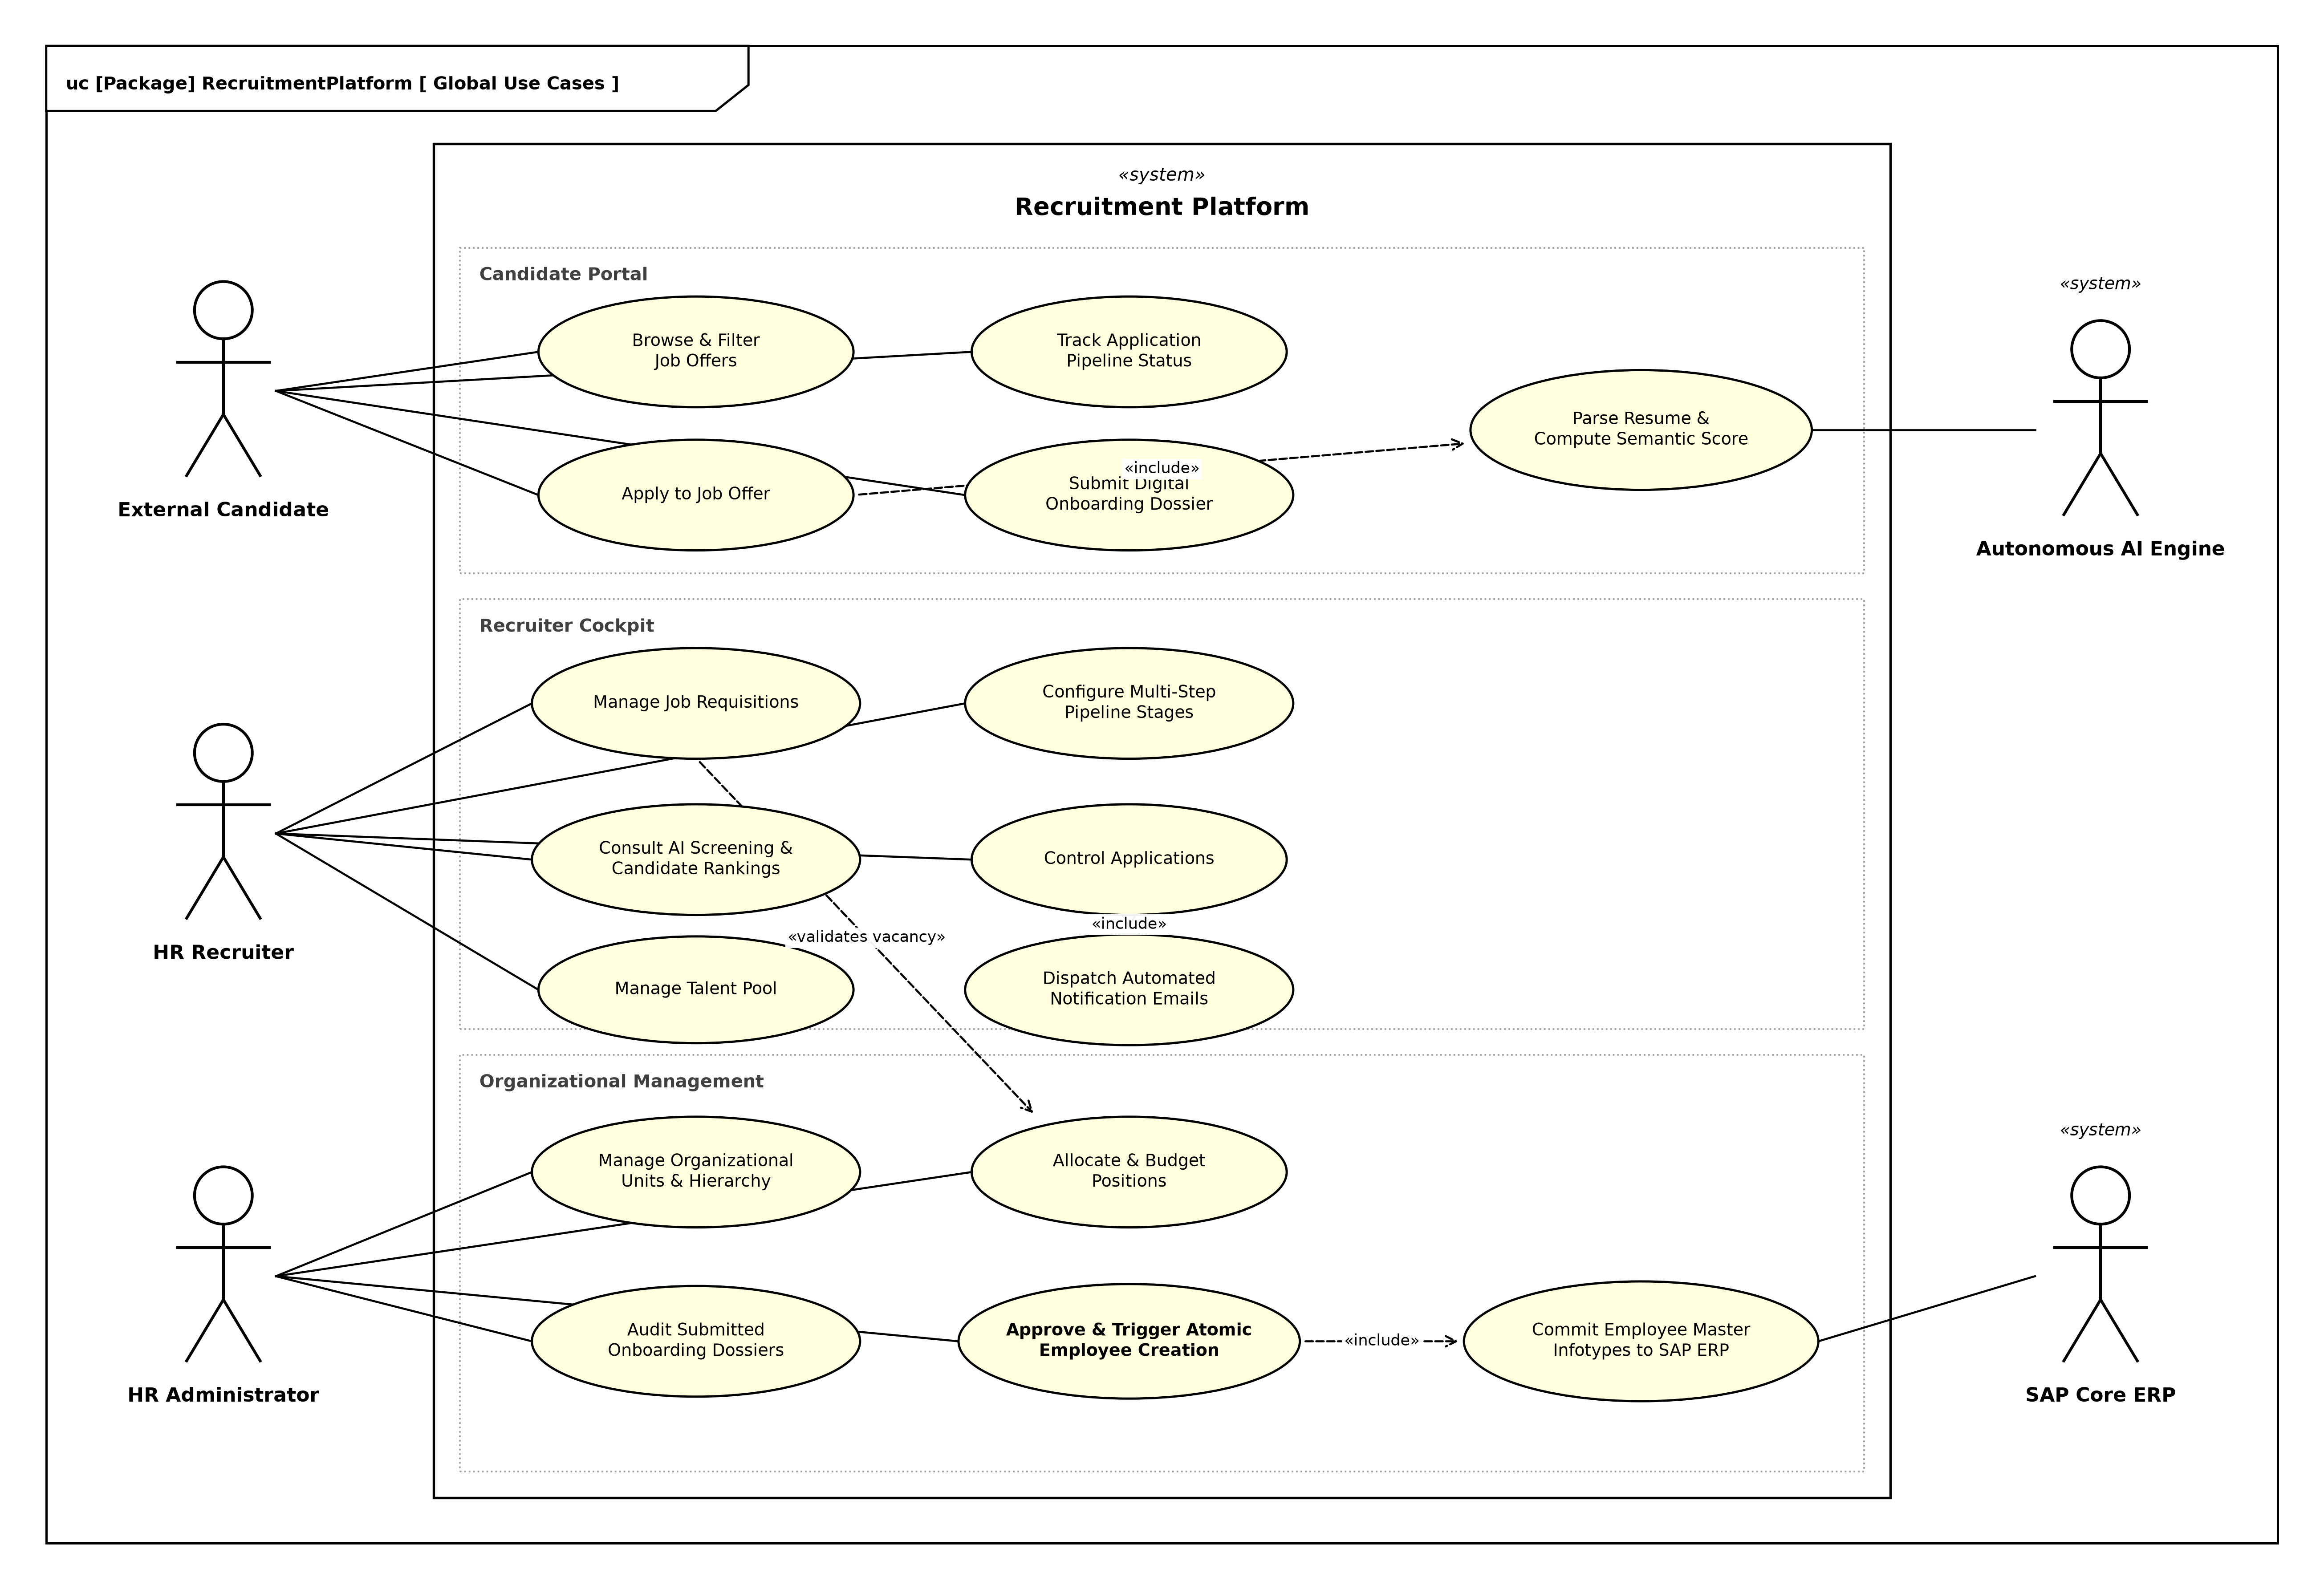
\includegraphics[width=15cm]{Figures/use_case_diagram.png}
    \caption{Global System Use Case Diagram}
    \label{fig:use_case_diagram}
\end{figure}

\subsubsection{User Stories}

\textbf{External Candidate:} Discovers a published job offer $\rightarrow$ submits application with resume $\rightarrow$ tracks real-time pipeline progression $\rightarrow$ completes onboarding dossier upon acceptance.

\textbf{HR Recruiter:} Creates job requisition in draft mode $\rightarrow$ configures pipeline stages and publishes $\rightarrow$ consults AI-generated candidate rankings $\rightarrow$ advances or rejects applicants through each stage.

\textbf{HR Administrator:} Models organizational hierarchy and creates vacant positions $\rightarrow$ audits submitted onboarding dossiers $\rightarrow$ triggers atomic employee creation $\rightarrow$ position status updates from Vacant to Filled.

% ─────────────────────────────────────────────
\section*{Conclusion}
\addcontentsline{toc}{section}{Conclusion}
% ─────────────────────────────────────────────

This chapter analyzed the existing recruitment landscape, compared it with our platform in a comparative synthesis, and established a complete specification of functional and non-functional requirements with global use case modeling. The next chapter details the architecture and the design of the solution.